
Cet exercice est un questionnaire à choix multiples (QCM). Aucune justification n'est demandée.

Pour chaque question, quatre réponses (\textbf{A}, \textbf{B}, \textbf{C} ou \textbf{D}) sont proposées.

Une seule réponse est exacte. Recopier sur la copie le numéro de la question et la lettre correspondant à la réponse exacte.

\subsection*{Question 1}
Le prix de 3 melons est $8,40 $~\euro{}. Combien coûtent 5 melons?

\medskip

\begin{tabularx}{\linewidth}{|*{4}{>{\centering \arraybackslash}X|}}\hline
\textbf{Réponse A}&\textbf{Réponse B}&\textbf{Réponse C}&\textbf{Réponse D}\\ \hline
	$16,40 $~\euro{} & $42 $~\euro{} & $14 $~\euro{} & $10,40 $~\euro{}
\\ \hline
\end{tabularx}

\bigskip

\begin{minipage}[t]{0.5\linewidth}	\subsection*{Question 2}
Quelle transformation permet de passer de la figure 1 à la figure 2 ?
\end{minipage}
\hfill
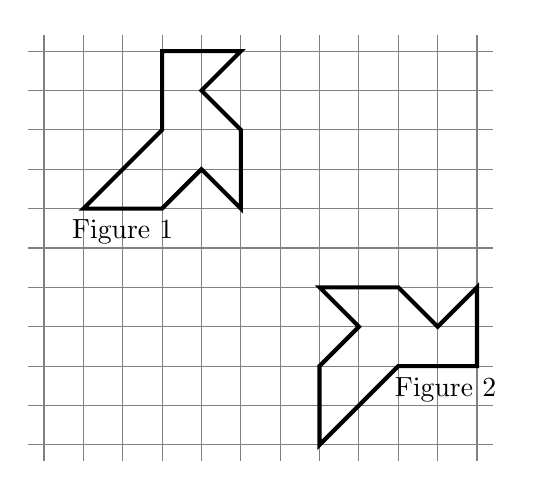
\begin{tikzpicture}[baseline={(T.south)}]
\draw[gray,line width=0.4pt,step=0.5] (-0.7,-0.2) grid (5.2,5.2);
\draw[line width=1.5pt] (0,3) --(1,3) node[pos=0.5,below]{Figure 1} --(1.5,3.5) --(2,3) --(2,4) --(1.5,4.5) --(2,5) --(1,5)node[above left,white](T){.} --(1,4) -- cycle;

\draw[line width=1.5pt] (3,0) --(3,1) --(3.5,1.5) --(3,2) --(4,2) --(4.5,1.5) --(5,2) --(5,1) --(4,1)node[pos = 0.4,below] {Figure 2} -- cycle;
\end{tikzpicture}

\medskip

\begin{tabularx}{\linewidth}{|*{4}{>{\centering \arraybackslash}X|}}\hline
\textbf{Réponse A}&\textbf{Réponse B}&\textbf{Réponse C}&\textbf{Réponse D}\\ \hline
Une symétrie centrale & Une rotation & Une translation & Une symétrie axiale \\ \hline
\end{tabularx}

\subsection*{Question 3}

Un article coûte $350 $~\euro{}. Son prix augmente de $20 \%$. Quel est son nouveau prix?

\medskip

\begin{tabularx}{\linewidth}{|*{4}{>{\centering \arraybackslash}X|}}\hline
\textbf{Réponse A}&\textbf{Réponse B}&\textbf{Réponse C}&\textbf{Réponse D}\\ \hline
$420 $~\euro{} & $330 $~\euro{} & $370 $~\euro{} & $280 $~\euro{}\\	\hline
\end{tabularx}

\bigskip

\begin{minipage}[t]{0.5\linewidth}
\subsection*{Question 4}
Quelle est l'aire du triangle rectangle ABC ?
\end{minipage}
\hfill
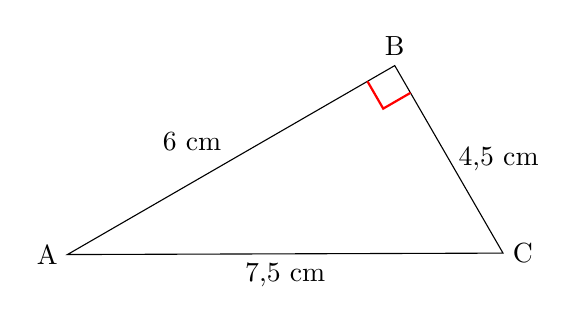
\begin{tikzpicture}[baseline={(B.base)}]
	\coordinate (A) at (210:4.8);
	\coordinate (B) at (0,0);
	\coordinate (C) at (-60:2.75);
	\node[left] at (A) {A};
	\node[above] at (B) {B};
	\node[right] at (C) {C};
	\draw (A) -- (B) node[pos=0.5,above left] {6 cm} -- (C) node[pos=0.5,right] {4,5 cm} -- cycle node[pos=0.5, below]{7,5 cm} ;
	\draw[red,line width = 0.8pt, rotate=30] (-0.4,0)--(-0.4,-0.4)--(0,-0.4) ;
	\end{tikzpicture}

	\medskip

\begin{tabularx}{\linewidth}{|*{4}{>{\centering \arraybackslash}X|}}\hline
\textbf{Réponse A}&\textbf{Réponse B}&\textbf{Réponse C}&\textbf{Réponse D}\\ \hline
$27 \mathrm{~cm}^{2}$ & $13,5 \mathrm{~cm}^{2}$ & $18 \mathrm{~cm}^{2}$ & $9 \mathrm{~cm}^{2}$ \\	\hline
\end{tabularx}

\subsection*{Question 5}

Quelle est la forme développée et réduite de l'expression $(2 x+3)(x-4)$ ?

\medskip

\begin{tabularx}{\linewidth}{|*{4}{>{\centering \arraybackslash}X|}}\hline
\textbf{Réponse A}&\textbf{Réponse B}&\textbf{Réponse C}&\textbf{Réponse D}\\ \hline
$2 x^{2}-5 x-12$ & $2 x^{2}-11 x-12$ & $2 x^{2}-12$ & $3 x-1$ \\ \hline
\end{tabularx}

\bigskip

\begin{minipage}[t]{0.61\linewidth}
\subsection*{Question 6}
Quel est le volume de cette pyramide à base rectangulaire ?
\end{minipage}
\hfill
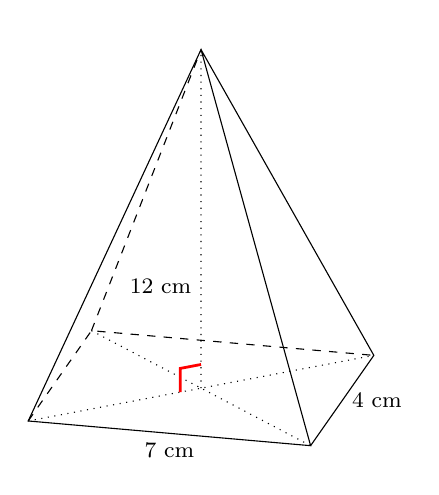
\begin{tikzpicture}[x=(-5:18mm),y=(55:7mm),z=(90:43mm),baseline={(T.base)}]
	\draw (0,0,0)--(2,0,0) node[pos=0.5,below]{{\footnotesize 7 cm}} --(1,1,1)node[above,white](T){.} --cycle
	(2,0,0) --(2,2,0) node[pos=0.5,right]{{\footnotesize 4 cm}}--(1,1,1);
	\draw[dotted](1,1,0)--(1,1,1)node[pos=0.3,left] {{\footnotesize 12 cm}} (0,0,0)--(2,2,0) (0,2,0)--(2,0,0);
	\draw[dashed] (0,0,0)--(0,2,0)--(2,2,0) (0,2,0)--(1,1,1);
	\draw[red,shift={(1,1,0)},line width=1pt] (-0.12,-0.12,0)--(-0.12,-0.12,0.07)--(0,0,0.07);
\end{tikzpicture}

\medskip

\begin{tabularx}{\linewidth}{|*{4}{>{\centering \arraybackslash}X|}}\hline
\textbf{Réponse A}&\textbf{Réponse B}&\textbf{Réponse C}&\textbf{Réponse D}\\ \hline
\np[cm^3]{23} & \np[cm^3]{112} & \np[cm^3]{336} & \np[cm^3]{168} \\	\hline
\end{tabularx}

\bigskip

